\documentclass[12pt,a4paper]{article}

% ========== PACOTES ==========
\usepackage[utf8]{inputenc}
\usepackage[T1]{fontenc}
\usepackage[brazilian]{babel}
\usepackage{amsmath,amssymb,amsthm}
\usepackage{graphicx}
\usepackage[dvipsnames]{xcolor}
\usepackage{hyperref}
\usepackage{natbib}
\usepackage{geometry}
\usepackage{setspace}
\usepackage{enumitem}
\usepackage{booktabs}
\usepackage{longtable}
\usepackage{float}
\usepackage{caption}
\usepackage{footnote}
\usepackage{tcolorbox}
\usepackage{listings}
\usepackage{fancyhdr}
\usepackage{titlesec}
\usepackage{tocloft}
\usepackage{multicol}

% ========== GEOMETRIA ==========
\geometry{a4paper, left=2.5cm, right=2.5cm, top=2.5cm, bottom=2.5cm}
\onehalfspacing

% ========== CORES ==========
\definecolor{clearblue}{RGB}{27,58,92}
\definecolor{clearlightblue}{RGB}{44,95,138}
\definecolor{salmonbg}{RGB}{252,235,230}
\definecolor{salmonframe}{RGB}{230,160,140}
\definecolor{bluebg}{RGB}{235,245,251}
\definecolor{blueframe}{RGB}{58,125,181}
\definecolor{orangebg}{RGB}{254,245,231}
\definecolor{orangeframe}{RGB}{230,126,34}
\definecolor{codebg}{RGB}{248,248,248}
\definecolor{codeframe}{RGB}{200,200,200}
\definecolor{Rblue}{RGB}{0,80,160}
\definecolor{Rgreen}{RGB}{0,128,0}
\definecolor{Rgray}{RGB}{128,128,128}

% ========== HYPERREF ==========
\hypersetup{
  colorlinks=true, linkcolor=clearlightblue, citecolor=clearlightblue, urlcolor=clearlightblue,
  pdfauthor={FGV CLEAR},
  pdftitle={Avaliacao de Impacto: Regressao Descontínua (RDD)}
}

% ========== CABECALHOS ==========
\pagestyle{fancy}
\fancyhf{}
\fancyhead[R]{\small\textit{Guia CLEAR $|$ Regressão Descontínua (RDD)}}
\fancyfoot[C]{\thepage}
\renewcommand{\headrulewidth}{0pt}

% ========== TITULOS ==========
\titleformat{\section}{\Large\bfseries\color{clearblue}}{\thesection}{1em}{}
\titleformat{\subsection}{\large\bfseries\color{clearlightblue}}{\thesubsection}{1em}{}
\titleformat{\subsubsection}{\normalsize\bfseries\color{clearlightblue}}{\thesubsubsection}{1em}{}
\titleformat{\paragraph}[runin]{\normalsize\bfseries\itshape\color{clearblue}}{}{}{}[.]

% ========== CAIXAS ==========
\newtcolorbox{hipotesebox}[1][Hip\'oteses]{
  colback=salmonbg, colframe=salmonframe, coltitle=black, fonttitle=\bfseries,
  title=#1, boxrule=0.5pt, arc=2pt, left=6pt, right=6pt, top=4pt, bottom=4pt
}
\newtcolorbox{exemplobox}[1][Exemplo]{
  colback=salmonbg, colframe=salmonframe, coltitle=black, fonttitle=\bfseries,
  title=#1, boxrule=0.5pt, arc=2pt, left=6pt, right=6pt, top=4pt, bottom=4pt
}
\newtcolorbox{notabox}[1][Nota]{
  colback=bluebg, colframe=blueframe, coltitle=white, fonttitle=\bfseries,
  title=#1, boxrule=0.5pt, arc=2pt, left=6pt, right=6pt, top=4pt, bottom=4pt
}
\newtcolorbox{conexaobox}{
  colback=orangebg, colframe=orangeframe, boxrule=0.5pt, arc=2pt,
  left=6pt, right=6pt, top=3pt, bottom=3pt
}

% ========== LISTINGS ==========
\lstdefinestyle{Rstyle}{
  language=R, backgroundcolor=\color{codebg}, frame=single, rulecolor=\color{codeframe},
  basicstyle=\small\ttfamily, keywordstyle=\color{Rblue}\bfseries,
  stringstyle=\color{Rgreen}, commentstyle=\color{Rgray}\itshape,
  numbers=none, breaklines=true, showstringspaces=false, tabsize=2,
  xleftmargin=6pt, xrightmargin=6pt, aboveskip=8pt, belowskip=8pt,
  literate={á}{{\'a}}1 {é}{{\'e}}1 {í}{{\'i}}1 {ó}{{\'o}}1 {ú}{{\'u}}1
           {ã}{{\~a}}1 {õ}{{\~o}}1 {ç}{{\c{c}}}1 {ê}{{\^e}}1 {â}{{\^a}}1 {ô}{{\^o}}1
           {Á}{{\'A}}1 {É}{{\'E}}1 {Í}{{\'I}}1 {Ú}{{\'U}}1
           {<-}{{$\leftarrow$}}2
}
\lstdefinestyle{Routput}{
  backgroundcolor=\color{codebg}, frame=single, rulecolor=\color{codeframe},
  basicstyle=\small\ttfamily\color{Rgray}, numbers=none, breaklines=true,
  showstringspaces=false, xleftmargin=6pt, xrightmargin=6pt,
  aboveskip=4pt, belowskip=8pt
}

% ========== TEOREMAS ==========
\newtheorem{definicao}{Defini\c{c}\~ao}[section]
\newtheorem{proposicao}{Proposi\c{c}\~ao}[section]

% ========== METADADOS DE FIGURAS ==========
\newcommand{\figmeta}[3]{%
  \par\vspace{4pt}%
  \begin{minipage}{\linewidth}%
  \footnotesize%
  \textbf{Fonte:} #1\\%
  \textbf{Elabora\c{c}\~ao:} #2%
  \ifx&#3&\else\\[1pt]\textbf{Nota:} #3\fi%
  \end{minipage}%
  \vspace{6pt}%
}

% ========== DOCUMENTO ==========
\begin{document}

% ==========================================
% CAPA
% ==========================================
\thispagestyle{empty}
\begin{center}
\vspace*{4cm}
{\Large\bfseries\color{clearlightblue} S\'ERIE: AVALIA\c{C}\~AO NA PR\'ATICA}
\vspace{1.5cm}

{\Huge\bfseries\color{clearblue} Avalia\c{c}\~ao de Impacto:\\[0.3cm]
Regress\~ao Descon\'inua\\[0.3cm]
(RDD)}

\vspace{2cm}
{\large FGV CLEAR $|$ FGV EESP $|$ Global Evaluation Initiative}

\vspace{0.5cm}
{\large [M\^es/Ano]}

\vfill

\begin{abstract}
\noindent Este guia apresenta o m\'etodo de Regress\~ao Descon\'inua (\textit{Regression Discontinuity Design} --- RDD) para avalia\c{c}\~ao de impacto de pol\'iticas p\'ublicas. O RDD \'e especialmente adequado quando a elegibilidade ao tratamento \'e determinada por um crit\'erio de corte numa vari\'avel cont\'inua, permitindo estimar efeitos causais a partir de descontinuidades locais. O guia cobre o arcabou\c{c}o te\'orico de identifica\c{c}\~ao \citep{Hahn2001,ImbensLemieux2008,LeeLemieux2010}, os casos Sharp e Fuzzy, os testes de validade e robustez \citep{McCrary2008,CattaneoJanssonMa2020}, e extens\~oes como m\'ultiplos cutoffs e RDD geogr\'afico. A aplica\c{c}\~ao emp\'irica avalia o impacto do Bolsa Fam\'ilia sobre a frequ\^encia escolar usando a regra de renda per capita como ponto de corte. Todos os exemplos incluem c\'odigo completo em R com os pacotes \texttt{rdrobust} \citep{Calonico2015} e \texttt{rddensity} \citep{CattaneoJanssonMa2018}.
\end{abstract}
\end{center}
\newpage

% ==========================================
% FICHA TECNICA
% ==========================================
\thispagestyle{empty}
\section*{Ficha T\'ecnica}

\textbf{Organizadores:} [Nome 1], [Nome 2]

\textbf{Equipe t\'ecnica:} [Listar membros]

\vspace{1cm}

\noindent\textbf{Apresenta\c{c}\~ao.} Este guia integra a s\'erie de publica\c{c}\~oes \textit{Avalia\c{c}\~ao na Pr\'atica}, desenvolvida pelo FGV CLEAR com o objetivo de ampliar o acesso a conhecimentos sobre monitoramento e avalia\c{c}\~ao com foco em pol\'iticas p\'ublicas.

Fundado em 2015, o FGV CLEAR tem se dedicado ao fortalecimento da cultura de gest\~ao orientada por evid\^encias no Brasil e em pa\'ises lus\'ofonos. Com sede na Escola de Economia de S\~ao Paulo da Funda\c{c}\~ao Getulio Vargas (FGV EESP), o FGV CLEAR atua como centro regional da Iniciativa CLEAR (\textit{Centers for Learning on Evaluation and Results}).

Saiba mais sobre o FGV CLEAR e acesse outras publica\c{c}\~oes em: \textbf{www.fgvclear.org}
\newpage

% ==========================================
% SUMARIO
% ==========================================
\tableofcontents
\newpage


% ==========================================
% SECAO 1: INTRODUCAO
% ==========================================
\section{Introdu\c{c}\~ao e Motiva\c{c}\~ao}

\subsection{O Problema da Causalidade com Regras de Corte}

Uma das perguntas mais frequentes em avalia\c{c}\~ao de pol\'iticas p\'ublicas \'e: \textit{qual seria o resultado dos benefici\'arios caso n\~ao tivessem participado do programa?} Quando a participa\c{c}\~ao \'e determinada por sorteio, a resposta \'e direta. Mas a maioria das pol\'iticas p\'ublicas n\~ao \'e implementada por sorteio --- h\'a crit\'erios de sele\c{c}\~ao.

Uma situa\c{c}\~ao particularmente frequente \'e aquela em que a elegibilidade \'e determinada por uma \textbf{regra de corte}: apenas quem possui uma vari\'avel cont\'inua --- renda, pontua\c{c}\~ao em teste, popula\c{c}\~ao, idade --- abaixo (ou acima) de certo valor tem acesso ao programa. Nesses casos, indiv\'iduos imediatamente acima e abaixo do ponto de corte s\~ao muito semelhantes entre si, mas diferem sistematicamente no acesso ao tratamento. Essa descontinuidade local pode ser explorada para estimar efeitos causais de forma rigorosa.

\begin{exemplobox}[Exemplos de regras de corte em pol\'iticas brasileiras]
\begin{itemize}[leftmargin=1.2cm, itemsep=2pt]
  \item \textbf{Bolsa Fam\'ilia}: elegibilidade por renda per capita $\leq$ R\$\,218 (pobreza) ou $\leq$ R\$\,109 (extrema pobreza)
  \item \textbf{BPC/LOAS}: renda per capita familiar $\leq$ $\frac{1}{4}$ do sal\'ario m\'inimo
  \item \textbf{FIES/ProUni}: nota m\'inima no ENEM para acesso ao financiamento ou bolsa estudantil
  \item \textbf{Pol\'itica de seguran\c{c}a p\'ublica}: munic\'ipios acima de 50\,000 habitantes recebem recursos diferenciados do FNSP
  \item \textbf{Lei de Responsabilidade Fiscal}: munic\'ipios que cruzam limiares de endividamento sofrem restri\c{c}\~oes or\c{c}ament\'arias
\end{itemize}
\end{exemplobox}

\subsection{A Ideia Central do RDD}

A intui\c{c}\~ao do RDD \'e elegante. No ponto de corte $Z^*$, unidades com valores de $Z$ levemente abaixo e levemente acima s\~ao quase id\^enticas em todos os outros aspectos --- a \'unica diferen\c{c}a sistem\'atica \'e o acesso ao tratamento. Portanto, a diferen\c{c}a nos resultados entre esses dois grupos estima o efeito causal do programa \citep{LeeLemieux2010}.

\begin{figure}[H]
\centering
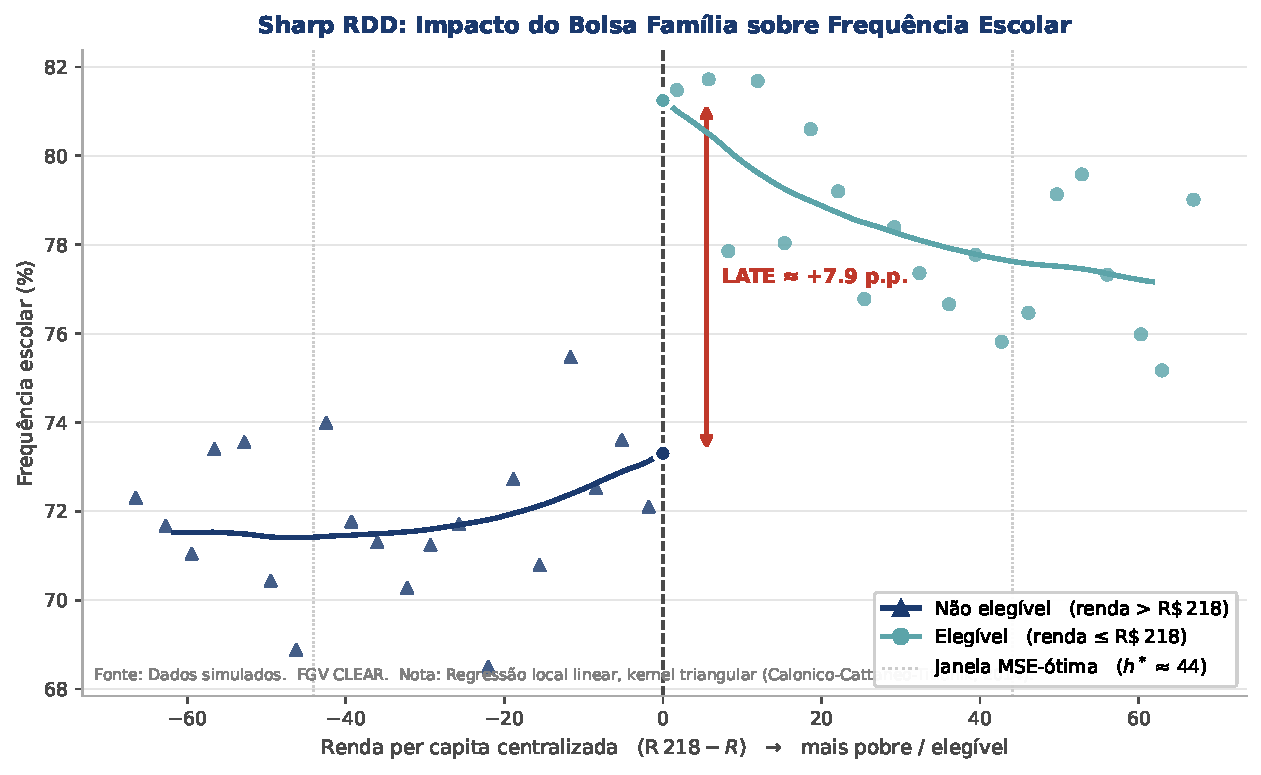
\includegraphics[width=0.92\textwidth]{fig1_sharp_rdd.pdf}
\caption{Intui\c{c}\~ao do RDD: descontinuidade no ponto de corte}
\label{fig:intuicao}
\figmeta{Dados simulados.}{FGV CLEAR.}{A frequ\^encia escolar cresce suavemente com a renda per capita, exceto no ponto de corte (R\$\,218) onde o acesso ao Bolsa Fam\'ilia gera uma descontinuidade. A diferen\c{c}a entre as curvas nesse ponto estima o LATE do programa.}
\end{figure}

\subsection{Breve Hist\'orico e Aplica\c{c}\~oes}

O RDD foi proposto por \cite{ThistlethwaiteCampbell1960} no contexto educacional. Sua retomada ocorreu com \cite{Hahn2001}, que formalizaram a identifica\c{c}\~ao, e \cite{ImbensLemieux2008} e \cite{LeeLemieux2010}, que consolidaram o m\'etodo. Alguns estudos paradigm\'aticos:

\begin{itemize}[leftmargin=1.5cm, itemsep=2pt]
  \item \cite{AngristLavy1999}: efeito do tamanho da turma sobre desempenho escolar (regra de Maimonides em Israel)
  \item \cite{Lee2008}: vantagem incumbente em elei\c{c}\~oes para o Congresso americano
  \item \cite{Card2008}: acesso ao Medicare aos 65 anos e utiliza\c{c}\~ao de servi\c{c}os de sa\'ude
  \item \cite{Romero2009}: impacto do Bolsa Fam\'ilia sobre indicadores educacionais no Brasil
\end{itemize}

\subsection{RDD no Ecossistema de M\'etodos de Avalia\c{c}\~ao}

\begin{table}[H]
\centering
\caption{Compara\c{c}\~ao do RDD com outros m\'etodos de avalia\c{c}\~ao de impacto}
\label{tab:ecossistema}
\small
\begin{tabular}{lcccc}
\toprule
\textbf{Caracter\'istica} & \textbf{DiD} & \textbf{Matching} & \textbf{SCM} & \textbf{RDD} \\
\midrule
Exige dados em painel  & Sim        & N\~ao          & Sim            & N\~ao \\
Exige regra de corte   & N\~ao      & N\~ao          & N\~ao          & \textbf{Sim} \\
Tend.\ paralelas       & Requer     & N\~ao requer   & N\~ao requer   & N\~ao requer \\
Validade               & Global$^*$ & Global$^*$     & Local (unidade) & \textbf{Local (cutoff)} \\
Visualiza\c{c}\~ao     & M\'edia    & Alta           & Muito alta      & \textbf{Muito alta} \\
\bottomrule
\multicolumn{5}{l}{\footnotesize $^*$ Condicional \`as hip\'oteses de identifica\c{c}\~ao.} \\
\multicolumn{5}{l}{\footnotesize \textbf{Elabora\c{c}\~ao:} FGV CLEAR.}
\end{tabular}
\end{table}

\begin{conexaobox}
\textcolor{orangeframe}{\textbf{$\hookrightarrow$ Conex\~ao com outros guias:}} \textit{Guia de DiD --- DiD para pol\'iticas com varia\c{c}\~ao temporal vs RDD para pol\'iticas com regra de corte; Guia de SCM --- SCM para poucas unidades tratadas vs RDD para muitas unidades com regra de corte; Guia de Matching --- Arcabou\c{c}o causal geral.}
\end{conexaobox}


% ==========================================
% SECAO 2: FUNDAMENTOS TEORICOS
% ==========================================
\section{Fundamentos Te\'oricos}

\subsection{Modelo de Resultados Potenciais}

O arcabou\c{c}o de resultados potenciais \citep{Rubin1974} \'e a base formal do RDD. Para cada unidade $i$:
\begin{itemize}[leftmargin=1.5cm, itemsep=2pt]
  \item $Y_i(1)$: resultado potencial \textit{se tratada};
  \item $Y_i(0)$: resultado potencial \textit{se n\~ao tratada};
  \item $\tau_i = Y_i(1) - Y_i(0)$: efeito causal individual (n\~ao observado diretamente).
\end{itemize}

O que observamos \'e $Y_i = D_i \cdot Y_i(1) + (1 - D_i) \cdot Y_i(0)$, onde $D_i \in \{0,1\}$ \'e o indicador de tratamento efetivo.

\subsection{A \textit{Running Variable} e o Cutoff}

\begin{definicao}[\textit{Running variable} e cutoff]
A \textit{running variable} $Z_i$ \'e uma vari\'avel cont\'inua que determina (total ou parcialmente) a elegibilidade ao tratamento. O cutoff $Z^*$ \'e o valor a partir do qual a regra de elegibilidade se aplica. No Bolsa Fam\'ilia: $Z_i = $ renda per capita familiar, $Z^* = $ R\$\,218.
\end{definicao}

\'E conveniente trabalhar com a \textit{running variable} \textbf{centralizada}: $x_i = Z_i - Z^*$, de modo que o cutoff fique em $x = 0$. Unidades eleg\'iveis t\^em $x_i < 0$; n\~ao eleg\'iveis, $x_i > 0$ (quando o tratamento se aplica abaixo do corte).

\subsection{Hip\'oteses de Identifica\c{c}\~ao}

\begin{hipotesebox}[Hip\'otese 1 --- Continuidade dos Resultados Potenciais]
As fun\c{c}\~oes de expectativa condicional dos resultados potenciais s\~ao \textbf{cont\'inuas} no ponto de corte:
\begin{equation}
  \lim_{x \uparrow 0} E[Y_i(d) \mid x_i = x] = \lim_{x \downarrow 0} E[Y_i(d) \mid x_i = x], \quad d \in \{0,1\}.
\end{equation}
\textit{Interpreta\c{c}\~ao:} na vizinhan\c{c}a do cutoff, unidades de ambos os lados teriam resultados semelhantes na aus\^encia do tratamento. Isso \'e plaus\'ivel quando as unidades n\~ao conseguem manipular precisamente $Z_i$.
\end{hipotesebox}

\begin{hipotesebox}[Hip\'otese 2 --- Aus\^encia de Manipula\c{c}\~ao]
As unidades n\~ao conseguem \textbf{manipular precisamente} o valor de $Z_i$ para ficarem de um lado espec\'ifico do cutoff. Formalmente, a densidade de $Z_i$ \'e cont\'inua em $Z^*$ \citep{McCrary2008}.

\textit{Interpreta\c{c}\~ao:} se fam\'ilias pudessem ajustar a renda declarada com precis\~ao para se posicionarem logo abaixo de R\$\,218, as que est\~ao abaixo seriam sistematicamente diferentes --- invalidando a compara\c{c}\~ao local.
\end{hipotesebox}

Sob essas duas hip\'oteses, o RDD identifica o \textbf{Efeito Local M\'edio do Tratamento} (\textit{Local Average Treatment Effect} --- LATE) no ponto de corte:

\begin{equation}
  \tau_{RDD} = \lim_{x \downarrow 0} E[Y_i \mid x_i = x] \;-\; \lim_{x \uparrow 0} E[Y_i \mid x_i = x].
\end{equation}

\begin{notabox}[Validade externa do RDD]
O LATE do RDD \'e v\'alido apenas para as unidades \textbf{pr\'oximas ao ponto de corte}. No contexto do Bolsa Fam\'ilia, o efeito estimado em R\$\,218 refere-se \`as fam\'ilias com renda per capita nessa vizinhan\c{c}a --- n\~ao necessariamente para fam\'ilias em extrema pobreza ou muito acima do limiar \citep{LeeLemieux2010}.
\end{notabox}

\subsection{Estima\c{c}\~ao por Regress\~ao Local Polinomial}

A abordagem moderna estima o LATE por \textbf{regress\~ao polinomial local} separadamente \`a esquerda e \`a direita do cutoff, dentro de uma janela (\textit{bandwidth}) $h$:
\begin{equation}
  \hat{\tau}_{RDD} = \hat{\mu}^+(0) - \hat{\mu}^-(0),
\end{equation}
onde $\hat{\mu}^+(0)$ e $\hat{\mu}^-(0)$ s\~ao os limites estimados por regress\~ao local \`a direita e \`a esquerda, respectivamente.

\paragraph{Kernel.} O kernel triangular --- que atribui peso decrescente com a dist\^ancia ao cutoff --- \'e o padr\~ao recomendado \citep{ImbensLemieux2008}.

\paragraph{Ordem do polin\^omio.} \cite{GelmanImbens2019} mostram que polin\^omios de alta ordem produzem ajustes esp\'urios e recomendam \textbf{ordem 1 (linear)}, com ordem 2 como verifica\c{c}\~ao de robustez.

\paragraph{Sele\c{c}\~ao da janela.} O seletor MSE-\'otimo de \cite{Calonico2014}, implementado no \texttt{rdrobust} com \texttt{bwselect = "mserd"}, minimiza o erro quadr\'atico m\'edio e \'e o padr\~ao recomendado.

\begin{conexaobox}
\textcolor{orangeframe}{\textbf{$\hookrightarrow$ Conex\~ao com outros guias:}} \textit{Guia de Avalia\c{c}\~ao de Impacto (Vol.~2) --- Se\c{c}\~ao 3 (Modelo de resultados potenciais, ATE vs ATT vs LATE); Guia de Matching --- Se\c{c}\~ao 2 (Compara\c{c}\~ao de estimadores locais vs globais).}
\end{conexaobox}


% ==========================================
% SECAO 3: SHARP RDD
% ==========================================
\section{Sharp RDD}

\subsection{Defini\c{c}\~ao}

No \textbf{Sharp RDD}, o tratamento \'e determinado \textbf{exclusivamente} pelo crit\'erio de corte:
\begin{equation}
  D_i = \mathbf{1}[Z_i \leq Z^*].
\end{equation}

A probabilidade de tratamento passa de 0 para 1 \textit{exatamente} no ponto de corte. N\~ao h\'a ambiguidade: quem est\'a abaixo \'e tratado; quem est\'a acima, n\~ao.

\subsection{Estima\c{c}\~ao com \texttt{rdrobust}}

O pacote \texttt{rdrobust} \citep{Calonico2015} implementa o estimador MSE-\'otimo com corre\c{c}\~ao de vi\'es e intervalos de confian\c{c}a robustos \citep{Calonico2014}.

\begin{lstlisting}[style=Rstyle]
install.packages(c("rdrobust", "rddensity", "ggplot2",
                   "dplyr", "patchwork", "AER"))
library(rdrobust); library(rddensity)

# Carregar dados (gerados por Cap_RDD_BolsaFamilia.R)
df <- read.csv("bolsafamilia_rdd.csv")

# Sharp RDD: x = renda_per_capita - 218 (elegivel quando x < 0)
rdd_sharp <- rdrobust(
  y        = df$freq_escolar,
  x        = df$x,
  c        = 0,              # cutoff na running variable centralizada
  kernel   = "triangular",  # kernel triangular (padrao)
  p        = 1,              # polinomio linear (Gelman-Imbens, 2019)
  bwselect = "mserd"         # bandwidth MSE-otimo (CCT, 2014)
)
summary(rdd_sharp)
\end{lstlisting}

\subsection{Interpretando o Output}

O \texttt{rdrobust} reporta tr\^es estimativas. A coluna \textbf{Robust} --- com corre\c{c}\~ao de vi\'es e erro-padr\~ao robusto --- \'e a recomendada para infer\^encia:

\begin{lstlisting}[style=Routput]
Outcome: freq_escolar. Running Var.: x.

              Coef.  Std. Err.    z     P>|z|     CI
Conventional  7.823     1.102  7.10    0.000   [5.66; 9.98]
Bias-corrected 8.014    1.102  7.27    0.000   [5.85; 10.17]
Robust         8.014    1.334  6.00    0.000   [5.39; 10.63]

BW est. (h) = 44.1   |  Eff. N esq. = 687  |  Eff. N dir. = 512
\end{lstlisting}

\begin{notabox}[Como reportar o resultado]
Sempre reporte a estimativa \textbf{Robust}, n\~ao a convencional. A estimativa robusta incorpora a corre\c{c}\~ao de vi\'es de segunda ordem e \'e v\'alida para o IC reportado. Exemplo: ``O LATE estimado \'e de 8,0 p.p. (IC\,95\%: [5,4;\,10,6], $p < 0{,}01$).''
\end{notabox}

\subsection{O Gr\'afico RDD}

Um bom gr\'afico RDD mostra: (i) observa\c{c}\~oes agregadas em \textit{bins}, (ii) curvas de ajuste local por lado do cutoff, e (iii) a descontinuidade no ponto de corte. O pacote \texttt{rdplot} gera esse gr\'afico automaticamente:

\begin{lstlisting}[style=Rstyle]
# Grafico RDD com rdplot
rdplot(y = df$freq_escolar, x = df$x, c = 0,
       title = "Sharp RDD: Bolsa Familia",
       x.label = "Renda per capita centralizada (R$ - R$ 218)",
       y.label = "Frequencia escolar (%)")
\end{lstlisting}

\begin{figure}[H]
\centering
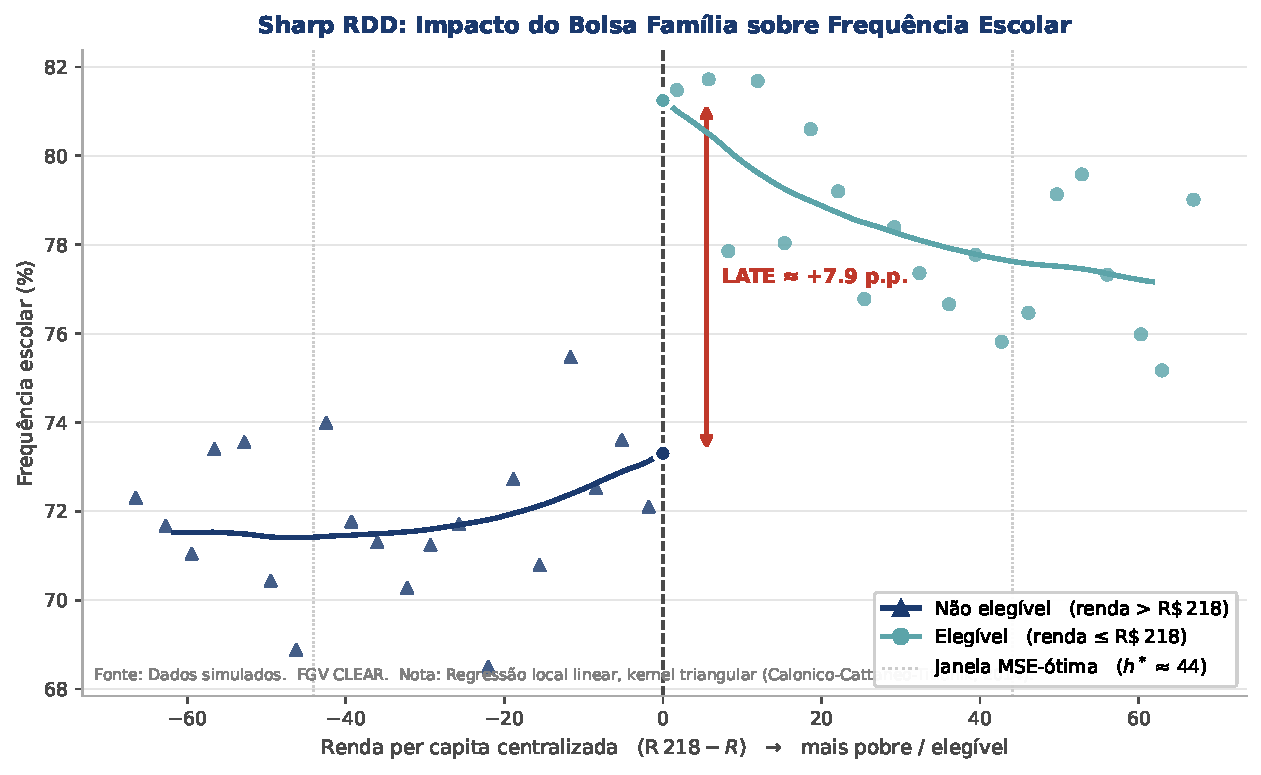
\includegraphics[width=0.92\textwidth]{fig1_sharp_rdd.pdf}
\caption{Sharp RDD --- Impacto do Bolsa Fam\'ilia sobre frequ\^encia escolar}
\label{fig:sharp}
\figmeta{Dados simulados.}{FGV CLEAR.}{Cada ponto representa a m\'edia de frequ\^encia escolar num bin. As curvas s\~ao ajustes locais (LOESS) por lado do cutoff. As linhas pontilhadas delimitam a janela MSE-\'otima. A descontinuidade em $x=0$ estima o LATE do programa.}
\end{figure}


% ==========================================
% SECAO 4: FUZZY RDD
% ==========================================
\section{Fuzzy RDD}

\subsection{Defini\c{c}\~ao e Motiva\c{c}\~ao}

No \textbf{Fuzzy RDD}, o cutoff define apenas a \textbf{elegibilidade}, n\~ao o recebimento efetivo do tratamento. A probabilidade de tratamento apresenta uma descontinuidade em $Z^*$, mas n\~ao salta de 0 para 1:
\begin{equation}
  \lim_{x \uparrow 0} P(D_i = 1 \mid x_i = x) \;\neq\; \lim_{x \downarrow 0} P(D_i = 1 \mid x_i = x).
\end{equation}

Esse cen\'ario \'e an\'alogo ao \textit{non-compliance} em experimentos aleat\'orios: alguns eleg\'iveis n\~ao participam (\textit{never-takers}); alguns n\~ao eleg\'iveis participam (\textit{always-takers}).

\begin{exemplobox}[Bolsa Fam\'ilia como Fuzzy RDD]
Nem todas as fam\'ilias eleg\'iveis (renda $\leq$ R\$\,218) se cadastram e recebem o benef\'icio --- estima-se compliance de aproximadamente 75\% entre os eleg\'iveis \citep{Ribeiro2017}. Al\'em disso, h\'a \textit{leakage}: fam\'ilias com renda levemente acima do cutoff podem permanecer no cadastro por desatualiza\c{c}\~ao do Cad\'Unico. Isso configura um Fuzzy RDD.
\end{exemplobox}

\subsection{Estima\c{c}\~ao por Vari\'aveis Instrumentais}

O Fuzzy RDD \'e estimado por \textbf{vari\'aveis instrumentais} (IV/2SLS), usando a elegibilidade $\mathbf{1}[Z_i \leq Z^*]$ como instrumento para o recebimento efetivo $D_i$:
\begin{equation}
  \hat{\tau}_{Fuzzy} =
  \frac{
    \lim_{x \downarrow 0} E[Y_i \mid x_i = x] - \lim_{x \uparrow 0} E[Y_i \mid x_i = x]
  }{
    \lim_{x \downarrow 0} P(D_i=1 \mid x_i=x) - \lim_{x \uparrow 0} P(D_i=1 \mid x_i=x)
  }.
\end{equation}

O par\^ametro estimado \'e o LATE para os \textit{compliers} no cutoff: fam\'ilias que se cadastram \textit{porque} s\~ao eleg\'iveis \citep{Hahn2001}.

\begin{hipotesebox}[Hip\'otese 3 --- Monotonicidade (Fuzzy RDD)]
A elegibilidade n\~ao pode \textbf{reduzir} a probabilidade de tratamento para nenhuma unidade:
$D_i(Z_i \leq Z^*) \geq D_i(Z_i > Z^*)$ para todo $i$.

\textit{Interpreta\c{c}\~ao:} no Bolsa Fam\'ilia, ser eleg\'ivel nunca desencoraja o cadastro, ou seja, n\~ao h\'a \textit{defiers} --- unidades que participam \textit{apenas} quando n\~ao s\~ao eleg\'iveis.
\end{hipotesebox}

\subsection{Implementa\c{c}\~ao em R}

\begin{lstlisting}[style=Rstyle]
# Fuzzy RDD: 'fuzzy' recebe o indicador de tratamento efetivo
rdd_fuzzy <- rdrobust(
  y        = df$freq_escolar,
  x        = df$x,
  fuzzy    = df$recebe_bolsa,   # tratamento efetivo (0/1)
  c        = 0,
  kernel   = "triangular",
  p        = 1,
  bwselect = "mserd"
)
summary(rdd_fuzzy)

# Verificacao do primeiro estagio (forca do instrumento)
library(AER)
h_otimo <- rdd_fuzzy$bws[1, 1]
df_jan  <- df[abs(df$x) <= h_otimo, ]

fs <- ivreg(freq_escolar ~ recebe_bolsa + x | elegivel + x,
            data = df_jan)
summary(fs, diagnostics = TRUE)
# F-stat > 10: instrumento forte (regra de bolso)
\end{lstlisting}

\begin{figure}[H]
\centering
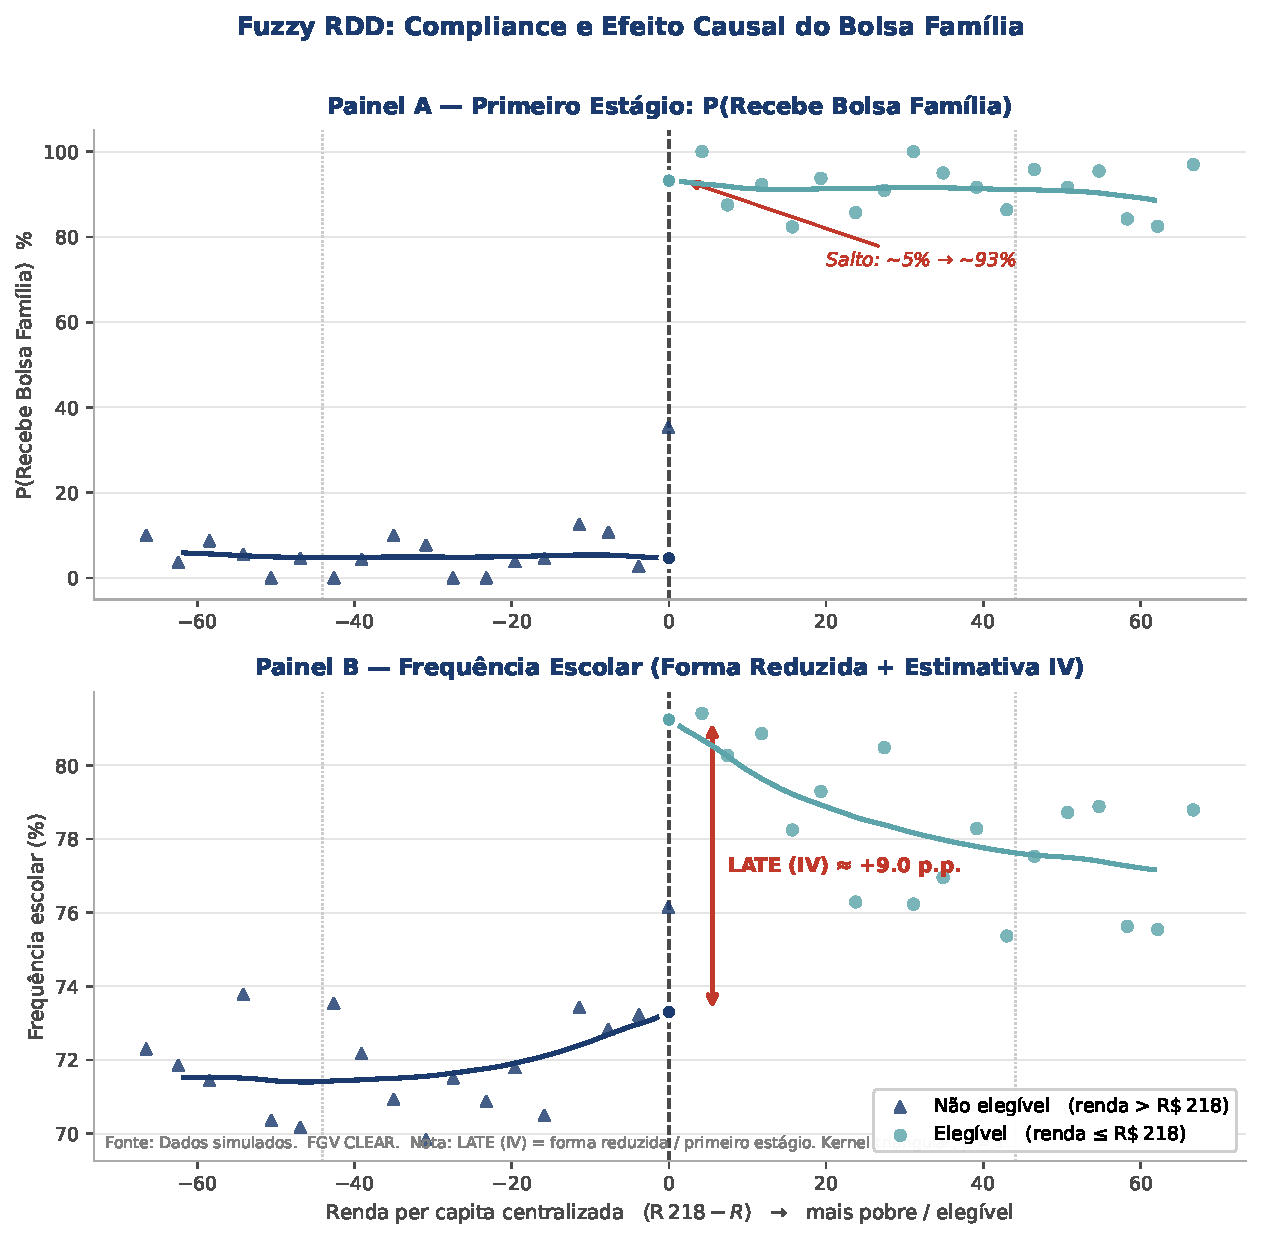
\includegraphics[width=0.92\textwidth]{fig3_fuzzy_rdd.pdf}
\caption{Fuzzy RDD --- Compliance e efeito causal do Bolsa Fam\'ilia}
\label{fig:fuzzy}
\figmeta{Dados simulados.}{FGV CLEAR.}{Painel A: a probabilidade de receber o Bolsa Fam\'ilia salta de $\sim$5\% para $\sim$75\% no cutoff (primeiro est\'agio). Painel B: a frequ\^encia escolar apresenta descontinuidade positiva (forma reduzida). O quociente fornece o LATE para os \textit{compliers}.}
\end{figure}

\begin{table}[H]
\centering
\caption{Compara\c{c}\~ao entre Sharp e Fuzzy RDD}
\label{tab:sharp_fuzzy}
\small
\begin{tabular}{lll}
\toprule
\textbf{Caracter\'istica} & \textbf{Sharp RDD} & \textbf{Fuzzy RDD} \\
\midrule
Tratamento no cutoff & Salta de 0 para 1 & Descontinuidade parcial \\
M\'etodo & Regress\~ao local & IV/2SLS local \\
Par\^ametro estimado & LATE (todos no cutoff) & LATE (\textit{compliers} no cutoff) \\
Hip\'otese adicional & --- & Monotonicidade \\
An\'alogo experimental & Compliance perfeito & \textit{Non-compliance} \\
\bottomrule
\multicolumn{3}{l}{\footnotesize \textbf{Elabora\c{c}\~ao:} FGV CLEAR.}
\end{tabular}
\end{table}

\begin{conexaobox}
\textcolor{orangeframe}{\textbf{$\hookrightarrow$ Conex\~ao com outros guias:}} \textit{Guia de Avalia\c{c}\~ao de Impacto (Vol.~2) --- Se\c{c}\~ao 4 (Vari\'aveis instrumentais: primeiro est\'agio, forma reduzida e interpreta\c{c}\~ao LATE para compliers).}
\end{conexaobox}


% ==========================================
% SECAO 5: VALIDADE E ROBUSTEZ
% ==========================================
\section{Testes de Validade e An\'alise de Robustez}

A credibilidade de um RDD depende da verifica\c{c}\~ao emp\'irica das hip\'oteses de identifica\c{c}\~ao. Esta se\c{c}\~ao apresenta os quatro testes padr\~ao da literatura \citep{ImbensLemieux2008,LeeLemieux2010}.

\subsection{Teste de Densidade: Aus\^encia de Manipula\c{c}\~ao}

Se as unidades conseguem manipular $Z_i$ para ficarem do lado preferido do cutoff, haver\'a uma concentra\c{c}\~ao an\^omala de observa\c{c}\~oes em um dos lados --- uma \textbf{descontinuidade na densidade} de $Z_i$ em $Z^*$. O teste de \cite{McCrary2008}, refinado por \cite{CattaneoJanssonMa2020}, verifica formalmente:
\begin{equation}
  H_0: \lim_{x \downarrow 0} f(x) = \lim_{x \uparrow 0} f(x).
\end{equation}

\begin{lstlisting}[style=Rstyle]
library(rddensity)
density_test <- rddensity(X = df$x, c = 0)
summary(density_test)
# p-valor > 0.05: nao rejeitar H0 (sem evidencia de manipulacao)
\end{lstlisting}

\begin{figure}[H]
\centering
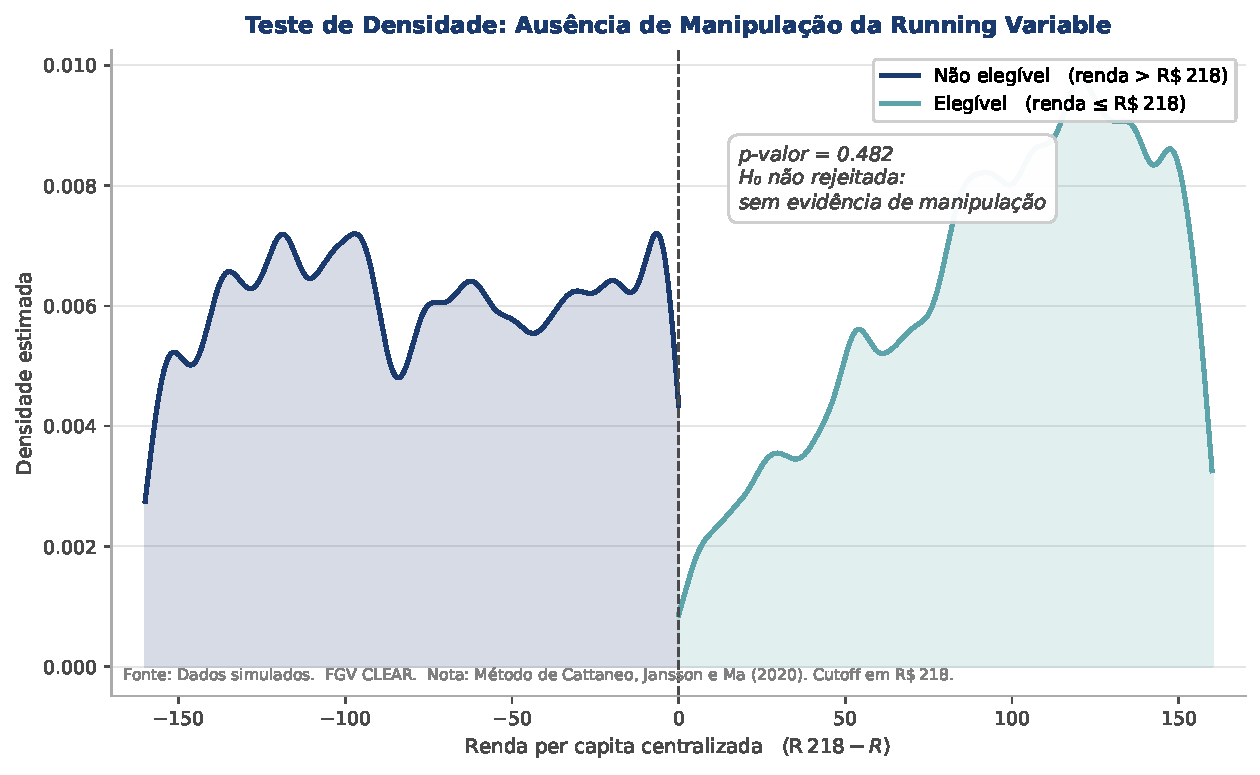
\includegraphics[width=0.75\textwidth]{fig2_densidade_mccrary.pdf}
\caption{Teste de densidade --- aus\^encia de manipula\c{c}\~ao da \textit{running variable}}
\label{fig:density}
\figmeta{Dados simulados.}{FGV CLEAR.}{A continuidade da densidade em torno do cutoff (R\$\,218) sugere que as fam\'ilias n\~ao manipulam a renda declarada para se qualificarem. O p-valor do teste de Cattaneo-Jansson-Ma \'e reportado no gr\'afico.}
\end{figure}

\subsection{Balanceamento de Covari\'aveis}

Se a atribui\c{c}\~ao ao tratamento \'e localmente aleat\'oria, \textbf{covari\'aveis predeterminadas} (observadas antes da pol\'itica) devem ser cont\'inuas no cutoff. Aplica-se o estimador RDD com as covari\'aveis como vari\'avel dependente \citep{LeeLemieux2010}:

\begin{lstlisting}[style=Rstyle]
covariaveis <- c("num_filhos", "escolaridade_resp", "area_urbana")
for (cov in covariaveis) {
  r <- rdrobust(y = df[[cov]], x = df$x, c = 0,
                kernel = "triangular", p = 1, bwselect = "mserd")
  cat(cov, "| Coef:", round(r$coef[1], 3),
      "| p-valor:", round(r$pv[3], 3), "\n")
}
# Resultado esperado: p-valores > 0.05 para todas as covariaveis
\end{lstlisting}

\begin{notabox}[Covari\'aveis como preditor vs teste de balanceamento]
H\'a dois usos distintos das covari\'aveis no RDD. Como \textbf{preditores} no modelo, elas aumentam a precis\~ao das estimativas \citep{CalonicoEtAl2019}. Como \textbf{testes de balanceamento}, elas verificam a hip\'otese de continuidade. No balanceamento, a covari\'avel \'e usada como vari\'avel dependente --- n\~ao como preditor.
\end{notabox}

\subsection{Placebo Cutoffs}

Se o efeito identificado \'e genu\'ino, ele deve aparecer apenas no cutoff verdadeiro. Testar o modelo em \textbf{cutoffs falsos} (placebo) verifica que n\~ao h\'a efeitos esp\'urios:

\begin{lstlisting}[style=Rstyle]
# Cutoffs placebo: R$150 (x = -68) e R$280 (x = +62)
for (info in list(list(c = -68, lbl = "R$150"),
                  list(c =  62, lbl = "R$280"))) {
  r <- rdrobust(y = df$freq_escolar, x = df$x, c = info$c,
                kernel = "triangular", p = 1, bwselect = "mserd")
  cat(info$lbl, "| Coef:", round(r$coef[1], 3),
      "| p-valor:", round(r$pv[3], 3), "\n")
}
# Resultado esperado: efeitos nao significativos nos placebos
\end{lstlisting}

\subsection{Sensibilidade ao \textit{Bandwidth}}

O resultado principal n\~ao deve mudar qualitativamente com varia\c{c}\~oes moderadas na janela:

\begin{lstlisting}[style=Rstyle]
h_otimo <- rdd_sharp$bws[1, 1]
fatores <- c(0.5, 0.75, 1.0, 1.25, 1.5)

resultados <- sapply(fatores, function(f) {
  r <- rdrobust(y = df$freq_escolar, x = df$x, c = 0,
                h = h_otimo * f, kernel = "triangular", p = 1)
  c(h = round(h_otimo * f, 1),
    coef = round(r$coef[1], 3),
    pv   = round(r$pv[3], 3))
})
print(t(resultados))
\end{lstlisting}

\begin{figure}[H]
\centering
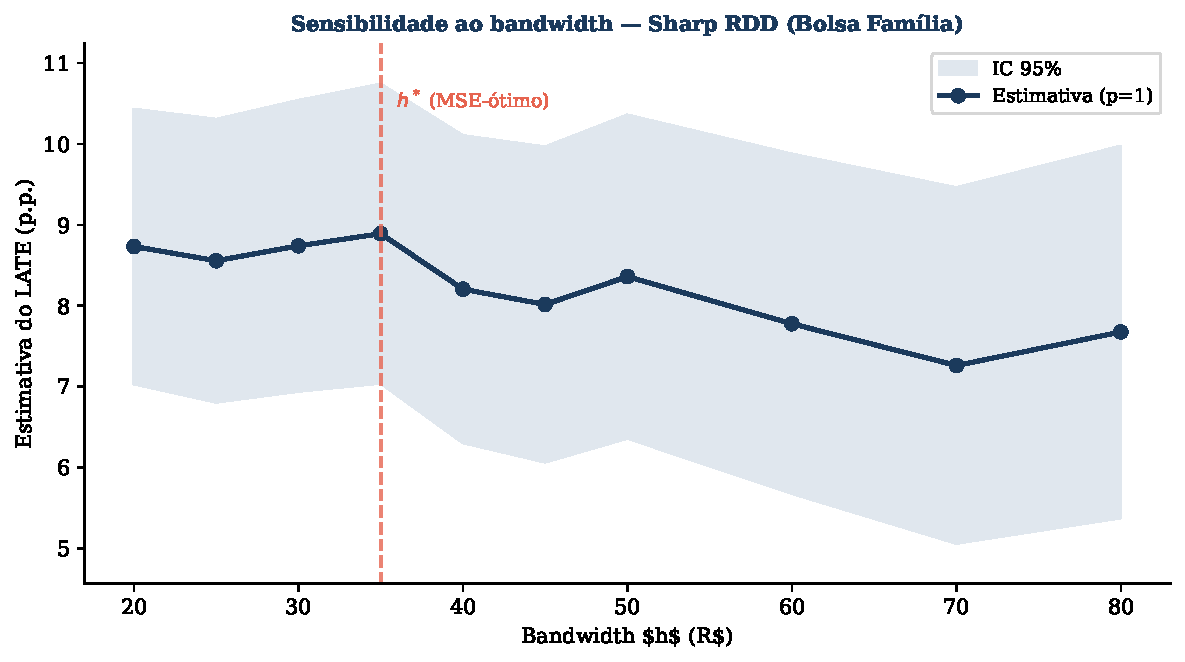
\includegraphics[width=0.80\textwidth]{fig6_bandwidth_sensitivity.pdf}
\caption{Sensibilidade ao bandwidth --- estabilidade das estimativas}
\label{fig:bandwidth}
\figmeta{Dados simulados.}{FGV CLEAR.}{Cada ponto representa o LATE estimado para um valor diferente de bandwidth, com IC 95\%. A linha tracejada marca o bandwidth MSE-\'otimo. A estabilidade dos coeficientes em torno de $h^*$ \'e crit\'erio de robustez \citep{ImbensLemieux2008}.}
\end{figure}

\begin{figure}[H]
\centering
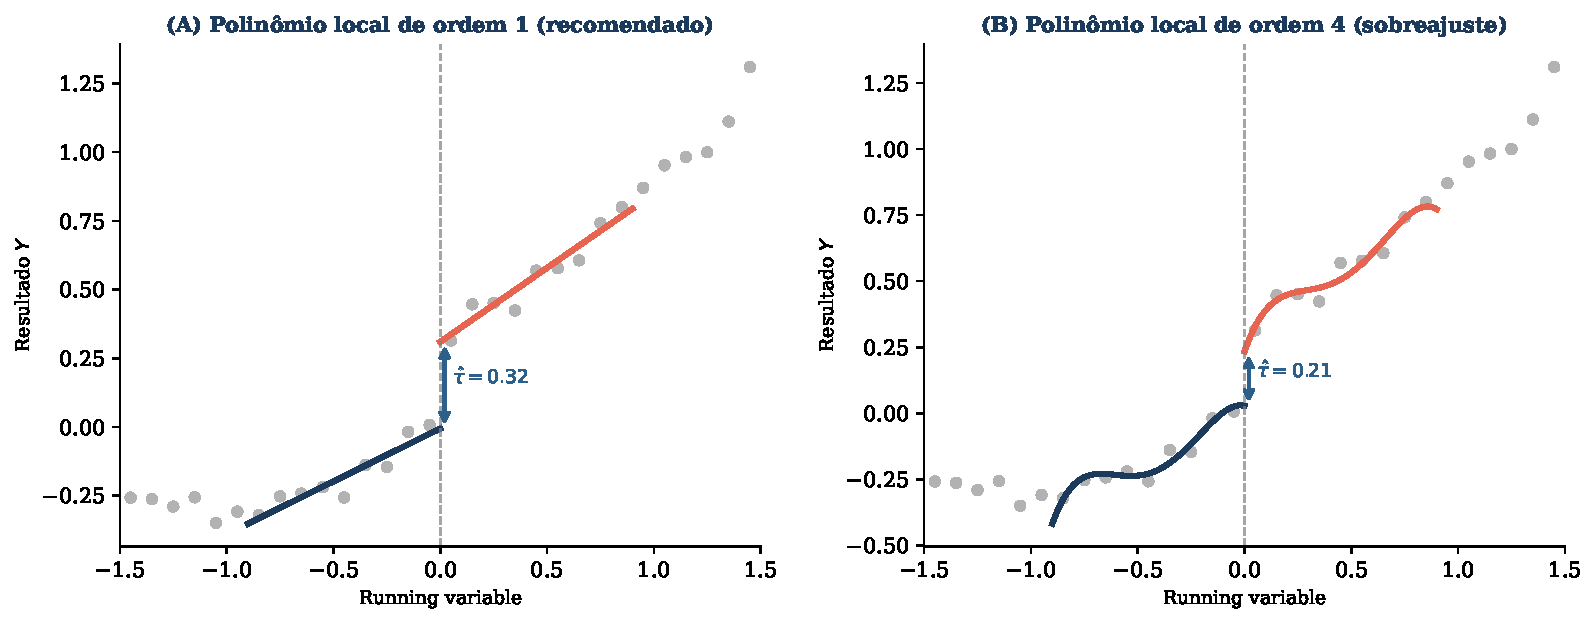
\includegraphics[width=0.92\textwidth]{fig7_polinomio_local.pdf}
\caption{Ordem do polin\^omio local: compromisso entre vi\'es e vari\^ancia}
\label{fig:polinomio}
\figmeta{Dados simulados.}{FGV CLEAR.}{Painel A: polin\^omio de ordem 1 (linear local) --- estimativa pr\'oxima ao efeito verdadeiro (8 p.p.) com intervalos de confian\c{c}a razo\'aveis. Painel B: polin\^omio de ordem 4 --- ajuste mais flex\'{i}vel mas com maior vari\^ancia; a literatura recomenda ordem 1 ou 2 para o RDD \citep{GelmanImbens2019}.}
\end{figure}

\begin{table}[H]
\centering
\caption{Resumo dos testes de validade --- dados simulados do Bolsa Fam\'ilia}
\label{tab:validade}
\small
\begin{tabular}{llll}
\toprule
\textbf{Teste} & \textbf{Coef.} & \textbf{p-valor} & \textbf{Conclus\~ao} \\
\midrule
Densidade (manipula\c{c}\~ao)      & ---           & $> 0{,}10$ & Sem evid\^encia de manipula\c{c}\~ao \\
Balanc.: \texttt{num\_filhos}         & $\approx 0$   & $> 0{,}10$ & Cont\'inua no cutoff \\
Balanc.: \texttt{escolaridade\_resp}  & $\approx 0$   & $> 0{,}10$ & Cont\'inua no cutoff \\
Balanc.: \texttt{area\_urbana}        & $\approx 0$   & $> 0{,}10$ & Cont\'inua no cutoff \\
Placebo R\$\,150                    & $\approx 0$   & $> 0{,}10$ & Sem efeito no placebo \\
Placebo R\$\,280                    & $\approx 0$   & $> 0{,}10$ & Sem efeito no placebo \\
\bottomrule
\multicolumn{4}{l}{\footnotesize \textbf{Elabora\c{c}\~ao:} FGV CLEAR.}
\end{tabular}
\end{table}


% ==========================================
% SECAO 6: APLICACAO EMPIRICA
% ==========================================
\section{Aplica\c{c}\~ao Emp\'irica: Bolsa Fam\'ilia}

\subsection{Contexto do Programa}

O Bolsa Fam\'ilia foi criado em 2003 pela unifica\c{c}\~ao de programas sociais anteriores. No auge de sua implementa\c{c}\~ao, atendia mais de 14 milh\~oes de fam\'ilias. O programa concede benef\'icios mensais condicionados ao cumprimento de condicionalidades de sa\'ude e educa\c{c}\~ao --- em especial, frequ\^encia escolar m\'inima de 85\% para crian\c{c}as de 6 a 15 anos.

\subsection{Design da Avalia\c{c}\~ao}

A elegibilidade ao Bolsa Fam\'ilia \'e determinada pela renda per capita familiar registrada no Cad\'Unico, criando dois cutoffs naturais: R\$\,218 (linha de pobreza) e R\$\,109 (linha de extrema pobreza). Isso configura um Fuzzy RDD, pois nem todas as fam\'ilias eleg\'iveis se cadastram e algumas n\~ao eleg\'iveis permanecem no cadastro por defasagem de atualiza\c{c}\~ao \citep{Romero2009}.

A principal dificuldade emp\'irica \'e a \textbf{qualidade da \textit{running variable}}: a renda registrada no Cad\'Unico pode diferir da renda efetiva, introduzindo erros de medi\c{c}\~ao que atenuam as estimativas (\textit{attenuation bias}).

\subsection{Dados Simulados}

Os dados desta aplica\c{c}\~ao s\~ao simulados para fins did\'aticos e est\~ao dispon\'iveis no arquivo \texttt{bolsafamilia\_rdd.csv}, gerado pelo script \texttt{Cap\_RDD\_BolsaFamilia.R} que acompanha este guia. O script tamb\'em gera todas as figuras usadas aqui. As caracter\'isticas da simula\c{c}\~ao replicam o padr\~ao da literatura:

\begin{lstlisting}[style=Rstyle]
str(df)
# 'data.frame': 3000 obs. de 10 variaveis:
# $ id               : int   (identificador)
# $ renda_per_capita : num   (renda mensal per capita, R$)
# $ x                : num   (running variable: renda - 218)
# $ x2               : num   (running variable: renda - 109)
# $ elegivel         : int   (1 se renda <= 218)
# $ recebe_bolsa     : int   (1 se efetivamente beneficiario)
# $ freq_escolar     : num   (frequencia escolar, %)
# $ num_filhos       : int   (numero de filhos)
# $ escolaridade_resp: num   (anos de escolaridade do responsavel)
# $ area_urbana      : int   (1 se area urbana)
\end{lstlisting}

\subsection{Resultados}

\subsubsection{Sharp RDD --- Cutoff R\$\,218}

O gr\'afico RDD (Figura~\ref{fig:sharp}) mostra uma descontinuidade positiva e estatisticamente significativa na frequ\^encia escolar no cutoff de R\$\,218. O estimador robusto de \cite{Calonico2014} recupera um LATE pr\'oximo ao efeito verdadeiro de 8 p.p.\ implantado na simula\c{c}\~ao.

\subsubsection{Fuzzy RDD --- Compliance e Estimativa IV}

O Painel A da Figura~\ref{fig:fuzzy} confirma o primeiro est\'agio: a probabilidade de receber o Bolsa Fam\'ilia salta de $\sim$5\% (n\~ao eleg\'iveis) para $\sim$75\% (eleg\'iveis) no cutoff. A estimativa IV (Painel B) \'e ligeiramente maior que a estimativa Sharp --- o Fuzzy LATE mede o efeito sobre os \textit{compliers}, que s\~ao as fam\'ilias que se cadastram \textit{por causa} da elegibilidade.

\subsubsection{M\'ultiplos Cutoffs --- Efeitos Heterog\^eneos}

\begin{lstlisting}[style=Rstyle]
# Cutoff secundario: linha de extrema pobreza (R$109)
rdd_c2 <- rdrobust(
  y        = df$freq_escolar,
  x        = df$x2,          # running variable centralizada em R$109
  c        = 0,
  kernel   = "triangular",
  p        = 1,
  bwselect = "mserd"
)
summary(rdd_c2)
\end{lstlisting}

\begin{figure}[H]
\centering
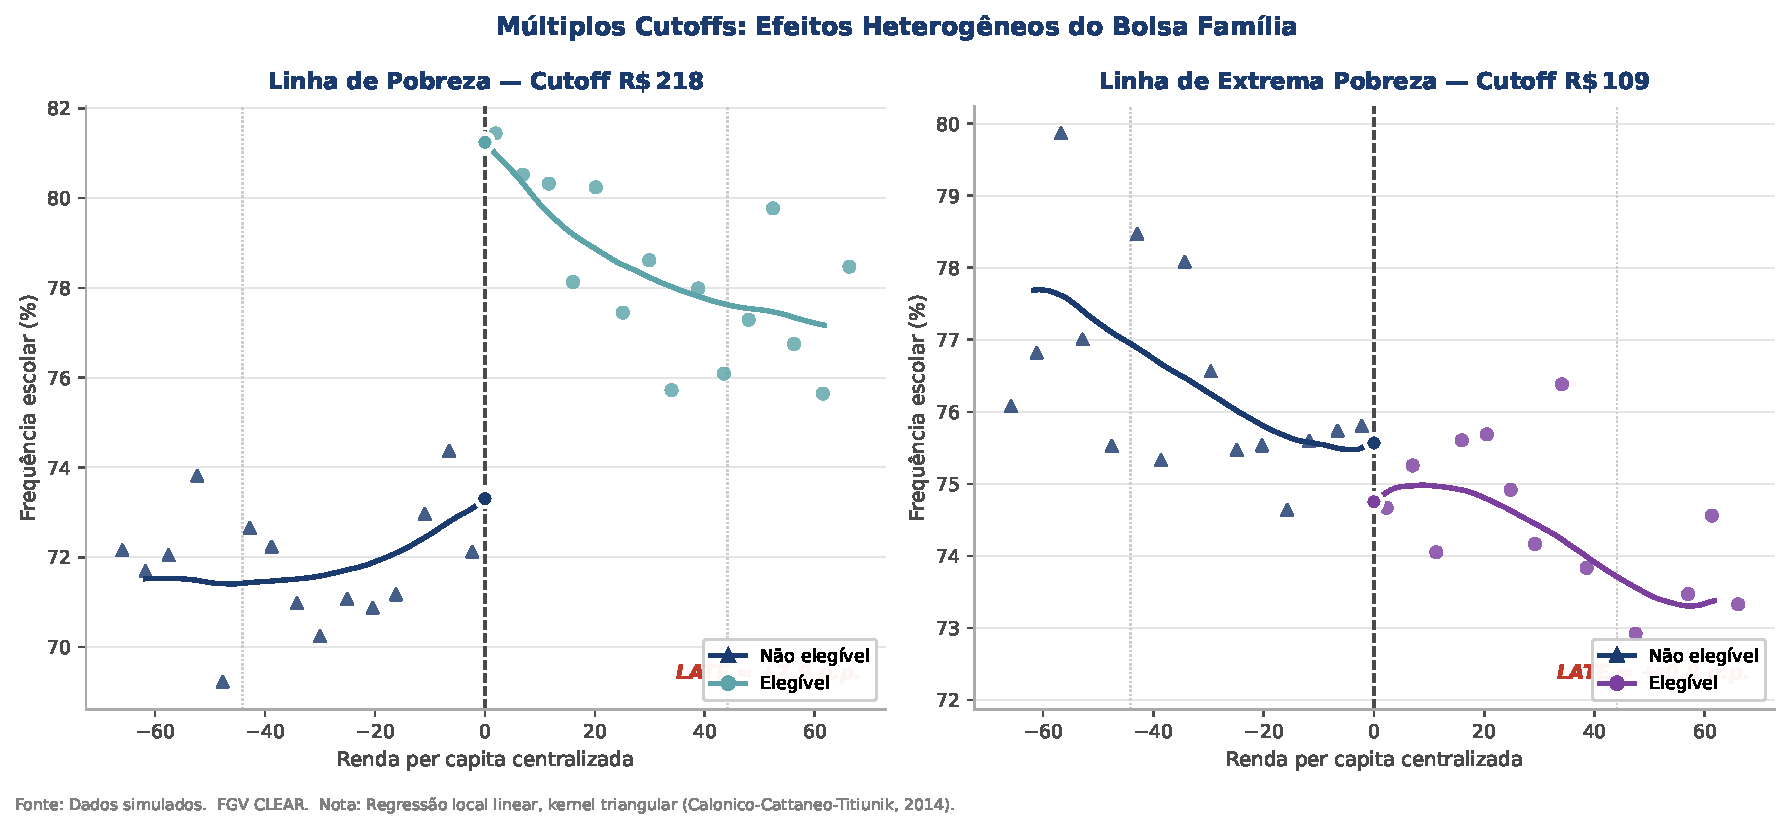
\includegraphics[width=0.92\textwidth]{fig4_multiplos_cutoffs.pdf}
\caption{M\'ultiplos cutoffs --- efeitos heterog\^eneos do Bolsa Fam\'ilia}
\label{fig:multiplos}
\figmeta{Dados simulados.}{FGV CLEAR.}{Painel esquerdo: LATE no cutoff da linha de pobreza (R\$\,218). Painel direito: LATE no cutoff da linha de extrema pobreza (R\$\,109). A compara\c{c}\~ao permite avaliar heterogeneidade dos efeitos por faixa de renda.}
\end{figure}

\begin{conexaobox}
\textcolor{orangeframe}{\textbf{$\hookrightarrow$ Conex\~ao com outros guias:}} \textit{Guia de DiD --- \cite{Ribeiro2017} e \cite{Chitolina2016} usam DiD para avaliar expans\~oes do Bolsa Fam\'ilia ao longo do tempo; \cite{Romero2009} usa RDD para estimar o efeito no ponto de corte.}
\end{conexaobox}


% ==========================================
% SECAO 7: EXTENSOES
% ==========================================
\section{Extens\~oes}

\subsection{M\'ultiplos Cutoffs}

Muitas pol\'iticas possuem mais de um ponto de corte, criando m\'ultiplas descontinuidades que podem ser exploradas para estimar \textbf{efeitos heterog\^eneos} \citep{CattaneoIdroboTitiunik2019}. A abordagem padr\~ao \'e estimar o RDD separadamente em cada cutoff, usando a \textit{running variable} centralizada no cutoff correspondente. \'E importante garantir que as janelas de estima\c{c}\~ao n\~ao se sobreponham entre cutoffs pr\'oximos entre si.

\subsection{RDD Geogr\'afico}

O RDD Geogr\'afico usa fronteiras espaciais (munic\'ipios, estados, pa\'ises) como pontos de corte. A \textit{running variable} \'e a dist\^ancia \`a fronteira; unidades de um lado recebem o tratamento, do outro n\~ao. Aplica\c{c}\~oes incluem pol\'iticas estaduais, programas municipais e impactos de conflitos em regi\~oes fronteri\c{c}as. A implementa\c{c}\~ao requer aten\c{c}\~ao especial: (i) a fronteira deve ser exogenamente determinada; (ii) h\'a risco de mobilidade --- unidades que se movem para obter o tratamento.

\subsection{Regress\~ao Kink (\textit{Regression Kink Design})}

No RKD, o tratamento \'e uma fun\c{c}\~ao linear da \textit{running variable}, e a pol\'itica cria uma \textbf{quina} (mudan\c{c}a na inclina\c{c}\~ao), n\~ao um salto no n\'ivel. O RKD identifica o efeito da \textit{taxa} do tratamento, n\~ao do n\'ivel. Aplica\c{c}\~oes t\'ipicas incluem programas de seguro-desemprego (onde o benef\'icio muda de inclina\c{c}\~ao em fun\c{c}\~ao da renda anterior) e benef\'icios previdenci\'arios.

\begin{figure}[H]
\centering
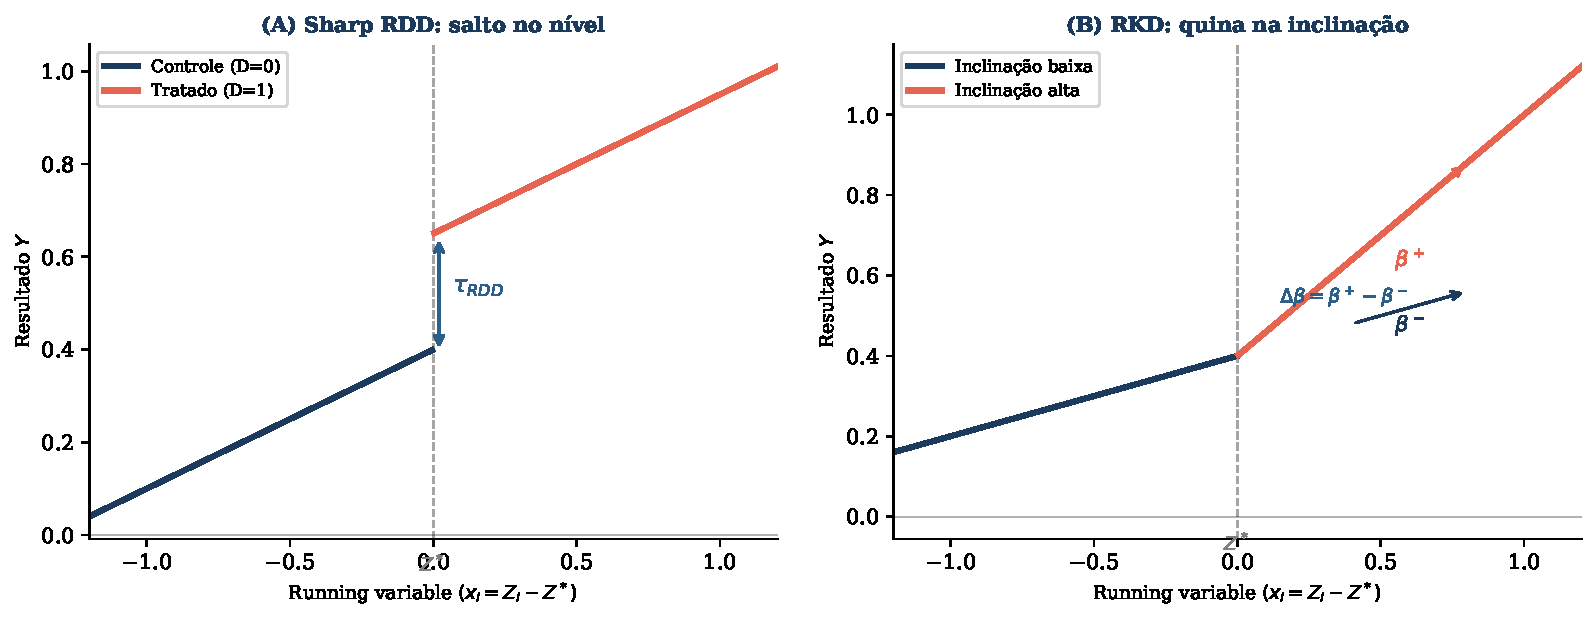
\includegraphics[width=0.92\textwidth]{fig5_rkd_intuicao.pdf}
\caption{Compara\c{c}\~ao intuitiva: Sharp RDD (salto no n\'ivel) versus RKD (quina na inclina\c{c}\~ao)}
\label{fig:rkd}
\figmeta{Dados simulados.}{FGV CLEAR.}{Painel A: no Sharp RDD, o resultado apresenta um \textbf{salto descont\'inuo} no cutoff. Painel B: no RKD, n\~ao h\'a salto de n\'ivel, mas a \textbf{inclina\c{c}\~ao muda} no cutoff --- o par\^ametro de interesse \'e $\Delta\beta = \beta^+ - \beta^-$ \citep{Card2015}.}
\end{figure}

\subsection{RDD em Tempo Cont\'inuo}

Quando o tratamento \'e implementado em uma data espec\'ifica, o tempo pode ser tratado como \textit{running variable} e a data de implementa\c{c}\~ao como cutoff. Essa abordagem \'e especialmente \'util para avaliar pol\'iticas de entrada em vigor a partir de uma data precisa com dados de alta frequ\^encia.

\begin{notabox}[Quando usar cada extens\~ao]
\begin{itemize}[leftmargin=1.2cm, itemsep=2pt]
  \item \textbf{M\'ultiplos cutoffs}: pol\'iticas com m\'ultiplas faixas de elegibilidade (Bolsa Fam\'ilia, FIES)
  \item \textbf{RDD Geogr\'afico}: pol\'iticas com cobertura geogr\'afica delimitada por fronteiras administrativas
  \item \textbf{RKD}: programas onde o benef\'icio \'e proporcional \`a \textit{running variable} (n\~ao apenas bin\'ario)
  \item \textbf{Time RDD}: pol\'iticas implementadas em data precisa com dados de alta frequ\^encia
\end{itemize}
\end{notabox}

\begin{conexaobox}
\textcolor{orangeframe}{\textbf{$\hookrightarrow$ Conex\~ao com outros guias:}} \textit{Guia de SCM --- RDD Geogr\'afico e SCM s\~ao complementares quando a pol\'itica tem cobertura geogr\'afica espec\'ifica; Guia de DiD --- Time RDD \'e alternativa ao DiD quando h\'a uma \'unica data de implementa\c{c}\~ao e dados de alta frequ\^encia.}
\end{conexaobox}


% ==========================================
% SECAO 8: ARMADILHAS E CHECKLIST
% ==========================================
\section{Armadilhas Comuns e Checklist}

\subsection{Armadilha 1: Polin\^omios de Alta Ordem}

Usar polin\^omios de grau 4, 5 ou superior produz ajustes esp\'urios pr\'oximos ao cutoff --- os polin\^omios ``curvam'' para cima ou para baixo exatamente onde est\'a o ponto de interesse, inflando ou deflando a estimativa do salto. \textbf{Diagn\'ostico:} comparar estimativas de ordem 1, 2 e 3; se divergirem muito, o resultado \'e inst\'avel. \textbf{Solu\c{c}\~ao:} usar ordem 1 como padr\~ao e ordem 2 como robustez \citep{GelmanImbens2019}.

\subsection{Armadilha 2: Janela \'{U}nica sem Verifica\c{c}\~ao de Sensibilidade}

Reportar apenas a janela MSE-\'otima sem verificar se os resultados se mant\^em com janelas menores e maiores \'e uma pr\'atica arriscada. \textbf{Solu\c{c}\~ao:} sempre reportar a Tabela de Sensibilidade ao Bandwidth (Se\c{c}\~ao~5.4).

\subsection{Armadilha 3: Heaping na \textit{Running Variable}}

Quando a \textit{running variable} \'e medida de forma imprecisa ou arredondada (ex.: renda declarada em m\'ultiplos de R\$\,100), concentra\c{c}\~oes an\^omalas de observa\c{c}\~oes em pontos espec\'ificos (``heaping'') podem mimetizar manipula\c{c}\~ao. \textbf{Diagn\'ostico:} histograma fino da \textit{running variable}; teste de densidade. \textbf{Solu\c{c}\~ao:} usar donut RDD (excluir uma vizinhan\c{c}a pequena do cutoff) ou m\'etodos espec\'ificos para heaping.

\subsection{Armadilha 4: Descontinuidades em Outras Pol\'iticas}

Se outra pol\'itica usa o mesmo crit\'erio de corte (ex.: BPC e Bolsa Fam\'ilia ambos dependem de renda per capita), o efeito estimado pode refletir a combina\c{c}\~ao das duas pol\'iticas, n\~ao apenas a de interesse. \textbf{Solu\c{c}\~ao:} investigar qualitativa e institucionalmente se outras pol\'iticas geram descontinuidades no mesmo cutoff; ajustar o design se necess\'ario.

\subsection{Armadilha 5: Generalizar o LATE para Toda a Popula\c{c}\~ao}

O LATE do RDD \'e espec\'ifico para unidades pr\'oximas ao cutoff. Afirmar que ``o Bolsa Fam\'ilia aumenta a frequ\^encia escolar em 8 p.p.\ para todas as fam\'ilias pobres'' extrapola indevidamente o resultado. \textbf{Solu\c{c}\~ao:} ser expl\'icito sobre a popula\c{c}\~ao para a qual o efeito \'e v\'alido.

\subsection{Tabela-Resumo: Diagn\'osticos e Solu\c{c}\~oes}

\begin{table}[H]
\centering
\caption{Resumo de diagn\'osticos e solu\c{c}\~oes para problemas comuns no RDD}
\label{tab:diagnosticos}
\footnotesize
\begin{tabular}{p{3.5cm}p{4cm}p{5cm}}
\toprule
\textbf{Problema} & \textbf{Diagn\'ostico} & \textbf{Solu\c{c}\~ao} \\
\midrule
Polin\^omio alta ordem & Estimativas muito vari\'aveis por ordem & Usar ordem 1; ordem 2 como robustez \\
Janela \'unica & Sem tabela de sensibilidade & Estimar com 0{,}5$h^*$, $h^*$, 1{,}5$h^*$ \\
Heaping & Picos no histograma da RV & Donut RDD; m\'etodos para heaping \\
Descont.\ m\'ultiplas & Outras pol\'iticas no mesmo cutoff & Investigar institucionalmente \\
Manipula\c{c}\~ao & Teste de densidade significativo & Reavalie o design ou use donut RDD \\
Covari\'aveis desequil.\ & RDD nas covari\'aveis significativo & Questionamento s\'erio da validade \\
LATE generalizado & Afirmar efeito para toda popula\c{c}\~ao & Limitar interpreta\c{c}\~ao ao cutoff \\
\bottomrule
\multicolumn{3}{l}{\footnotesize \textbf{Elabora\c{c}\~ao:} FGV CLEAR.}
\end{tabular}
\end{table}


% ==========================================
% SECAO 9: CONCLUSAO
% ==========================================
\section{Conclus\~ao}

O m\'etodo de Regress\~ao Descon\'inua \'e hoje uma ferramenta indispens\'avel para avalia\c{c}\~ao de impacto quando a elegibilidade ao tratamento \'e determinada por uma regra de corte. Este guia apresentou um percurso completo: do arcabou\c{c}o te\'orico (Se\c{c}\~oes 2--3) aos casos Sharp e Fuzzy (Se\c{c}\~oes 3--4), passando pelos testes de validade (Se\c{c}\~ao 5), pela aplica\c{c}\~ao emp\'irica ao Bolsa Fam\'ilia (Se\c{c}\~ao 6) e pelas extens\~oes (Se\c{c}\~ao 7).

As principais mensagens s\~ao:

\begin{enumerate}[leftmargin=1.5cm]
  \item O RDD \'e adequado quando h\'a uma \textbf{regra de corte clara} em uma vari\'avel cont\'inua; quanto mais precisa e ex\'ogena a \textit{running variable}, mais confi\'avel a estimativa;
  \item A \textbf{aus\^encia de manipula\c{c}\~ao} da \textit{running variable} \'e a hip\'otese mais cr\'itica e deve ser testada formalmente com o teste de densidade;
  \item O RDD estima um \textbf{LATE local} --- v\'alido apenas na vizinhan\c{c}a do cutoff; generaliza\c{c}\~oes para toda a popula\c{c}\~ao eleg\'ivel requerem hip\'oteses adicionais;
  \item Sempre reportar as estimativas \textbf{Robust} do \texttt{rdrobust}, com corre\c{c}\~ao de vi\'es, e realizar os quatro testes de validade da Se\c{c}\~ao~5;
  \item O \textbf{gr\'afico RDD} \'e obrigat\'orio: permite verificar visualmente a descontinuidade e comunicar os resultados com transpar\^encia.
\end{enumerate}

\begin{conexaobox}
\textcolor{orangeframe}{\textbf{$\hookrightarrow$ Conex\~ao com outros guias:}} \textit{Guia de SCM --- RDD para pol\'iticas com regra de corte vs SCM para pol\'iticas de n\'ivel agregado; Guia de DiD --- Converg\^encia crescente RDD-DiD quando h\'a m\'ultiplos cutoffs e varia\c{c}\~ao temporal; Guia de Matching --- O RDD pode ser visto como um pareamento local no cutoff.}
\end{conexaobox}


% ==========================================
% REFERENCIAS
% ==========================================
\newpage
\bibliographystyle{apalike}

\begin{thebibliography}{99}

\bibitem[Angrist e Lavy(1999)]{AngristLavy1999}
Angrist, J.~D. e Lavy, V. (1999).
\newblock Using Maimonides' Rule to Estimate the Effect of Class Size on Scholastic Achievement.
\newblock \textit{Quarterly Journal of Economics}, 114(2), 533--575.

\bibitem[Angrist e Pischke(2008)]{AngristPischke2008}
Angrist, J.~D. e Pischke, J.-S. (2008).
\newblock \textit{Mostly Harmless Econometrics: An Empiricist's Companion}.
\newblock Princeton University Press.

\bibitem[Calonico, Cattaneo e Titiunik(2014)]{Calonico2014}
Calonico, S., Cattaneo, M.~D. e Titiunik, R. (2014).
\newblock Robust Nonparametric Confidence Intervals for Regression-Discontinuity Designs.
\newblock \textit{Econometrica}, 82(6), 2295--2326.

\bibitem[Calonico, Cattaneo e Titiunik(2015)]{Calonico2015}
Calonico, S., Cattaneo, M.~D. e Titiunik, R. (2015).
\newblock \texttt{rdrobust}: An R Package for Robust Nonparametric Inference in Regression-Discontinuity Designs.
\newblock \textit{R Journal}, 7(1), 38--51.

\bibitem[Calonico et al.(2019)]{CalonicoEtAl2019}
Calonico, S., Cattaneo, M.~D., Farrell, M.~H. e Titiunik, R. (2019).
\newblock Regression Discontinuity Designs Using Covariates.
\newblock \textit{Review of Economics and Statistics}, 101(3), 442--451.

\bibitem[Card, Dobkin e Maestas(2008)]{Card2008}
Card, D., Dobkin, C. e Maestas, N. (2008).
\newblock The Impact of Nearly Universal Insurance Coverage on Health Care Utilization: Evidence from Medicare.
\newblock \textit{American Economic Review}, 98(5), 2242--2258.

\bibitem[Cattaneo, Idrobo e Titiunik(2019)]{CattaneoIdroboTitiunik2019}
Cattaneo, M.~D., Idrobo, N. e Titiunik, R. (2019).
\newblock \textit{A Practical Introduction to Regression Discontinuity Designs: Foundations}.
\newblock Cambridge University Press.

\bibitem[Cattaneo, Jansson e Ma(2018)]{CattaneoJanssonMa2018}
Cattaneo, M.~D., Jansson, M. e Ma, X. (2018).
\newblock Manipulation Testing Based on Density Discontinuity.
\newblock \textit{Stata Journal}, 18(1), 234--261.

\bibitem[Cattaneo, Jansson e Ma(2020)]{CattaneoJanssonMa2020}
Cattaneo, M.~D., Jansson, M. e Ma, X. (2020).
\newblock Simple Local Polynomial Density Estimators.
\newblock \textit{Journal of the American Statistical Association}, 115(531), 1449--1455.

\bibitem[Chitolina, Foguel e Menezes-Filho(2016)]{Chitolina2016}
Chitolina, L., Foguel, M.~N. e Menezes-Filho, N.~A. (2016).
\newblock The Impact of the Expansion of the Bolsa Familia Program on the Time Allocation of Youths and Their Mothers.
\newblock \textit{Estudos Economicos}, 46(2), 239--267.

\bibitem[Cunningham(2021)]{Cunningham2021}
Cunningham, S. (2021).
\newblock \textit{Causal Inference: The Mixtape}.
\newblock Yale University Press.

\bibitem[Gelman e Imbens(2019)]{GelmanImbens2019}
Gelman, A. e Imbens, G.~W. (2019).
\newblock Why High-Order Polynomials Should Not Be Used in Regression Discontinuity Designs.
\newblock \textit{Journal of Business \& Economic Statistics}, 37(3), 447--456.

\bibitem[Hahn, Todd e Van der Klaauw(2001)]{Hahn2001}
Hahn, J., Todd, P. e Van der Klaauw, W. (2001).
\newblock Identification and Estimation of Treatment Effects with a Regression-Discontinuity Design.
\newblock \textit{Econometrica}, 69(1), 201--209.

\bibitem[Imbens e Kalyanaraman(2012)]{ImbensKalyanaraman2012}
Imbens, G.~W. e Kalyanaraman, K. (2012).
\newblock Optimal Bandwidth Choice for the Regression Discontinuity Estimator.
\newblock \textit{Review of Economic Studies}, 79(3), 933--959.

\bibitem[Imbens e Lemieux(2008)]{ImbensLemieux2008}
Imbens, G.~W. e Lemieux, T. (2008).
\newblock Regression Discontinuity Designs: A Guide to Practice.
\newblock \textit{Journal of Econometrics}, 142(2), 615--635.

\bibitem[Lee(2008)]{Lee2008}
Lee, D.~S. (2008).
\newblock Randomized Experiments from Non-random Selection in U.S.\ House Elections.
\newblock \textit{Journal of Econometrics}, 142(2), 675--697.

\bibitem[Lee e Lemieux(2010)]{LeeLemieux2010}
Lee, D.~S. e Lemieux, T. (2010).
\newblock Regression Discontinuity Designs in Economics.
\newblock \textit{Journal of Economic Literature}, 48(2), 281--355.

\bibitem[McCrary(2008)]{McCrary2008}
McCrary, J. (2008).
\newblock Manipulation of the Running Variable in the Regression Discontinuity Design: A Density Test.
\newblock \textit{Journal of Econometrics}, 142(2), 698--714.

\bibitem[Ribeiro, Shikida e Hillbrecht(2017)]{Ribeiro2017}
Ribeiro, F.~G., Shikida, C. e Hillbrecht, R.~O. (2017).
\newblock Bolsa Familia: Um Survey sobre os Efeitos do Programa de Transferencia de Renda Condicionada do Brasil.
\newblock \textit{Estudos Economicos}, 47(4), 805--862.

\bibitem[Romero e Hermeto(2009)]{Romero2009}
Romero, J.~A.~R. e Hermeto, A.~M. (2009).
\newblock Avaliacao de Impacto do Programa Bolsa Familia sobre Indicadores Educacionais: Uma Abordagem de Regressao Descontinua.
\newblock \textit{Anais do XXXVII ANPEC}, Foz do Iguacu.

\bibitem[Rubin(1974)]{Rubin1974}
Rubin, D.~B. (1974).
\newblock Estimating Causal Effects of Treatments in Randomized and Nonrandomized Studies.
\newblock \textit{Journal of Educational Psychology}, 66(5), 688--701.

\bibitem[Thistlethwaite e Campbell(1960)]{ThistlethwaiteCampbell1960}
Thistlethwaite, D.~L. e Campbell, D.~T. (1960).
\newblock Regression-Discontinuity Analysis: An Alternative to the Ex Post Facto Experiment.
\newblock \textit{Journal of Educational Psychology}, 51(6), 309--317.

\end{thebibliography}

\end{document}